\section{Background and Motivation}
some text \ldots

\subsection{Architecture of Hyperledger Fabric}
some text \ldots

\par
\textbf{(1) Endorsement Phase.} some text \ldots

\par
\textbf{(2) Ordering Phase.} some text \ldots

\par
\textbf{(3) Validation Phase.} some text \ldots

\par
\textbf{(4) Commit Phase.} some text \ldots

\subsection{Motivation for Data Privacy}
\par
some text \ldots
\subsubsection{Use Case Study: Food Traceability}
In September 2006, there was an outbreak of food-borne illness caused by Escherichia coli~\cite{ecoil}
bacteria in 26 U.S. states. This outbreak was linked to bagged spinach. By October 6, 2006, 199 people had been
infected, including three people who died and 31 who suffered kidney failure. It took regulators two
weeks to conduct the backtrace and determine the exact source of the outbreak. During those two weeks,
many people got sick and tons of good spinach was unnecessarily discarded---wrongfully
wasted because we could not tell the good spinach from the bad~\cite{blockchain-for-business}.
An efficient food traceability mechanism is the key to reduce the backtrace time in such a scenario.
Traceability is the ability to track and record the movement of food products throughout a supply chain, which
includes growing, harvesting, packing, manufacturing, repacking, storage, distribution, and sale to the consumer.
With these information, it is possible to trace backward in the supply chain (usually to find the source of a
problem) as well as trace forward (usually to do a recall of contaminated products).
\par
Food Standards Australia New Zealand (FSANZ)~\cite{fs}, European Commission's food safety policy~\cite{eu-foodsafety},
and Food and Agriculture Organization of United Nations (FAO)~\cite{fao-traceability} provide various guidelines on what
records need be kept in order to enable food traceability. The following are some of the records:
\begin{enumerate}[topsep=0pt,noitemsep,leftmargin=15pt]
	\item name and address (and other contact details) of suppliers/farmers and a description of products or inputs supplied.
	\item the name and contact information of the logistics providers and a description of products transpoted.
	\item name and addresses (and other contact details) of customers and a description of the product supplied to them along with the product ID.
    \item date of transaction or delivery.
    \item batch or lot identification (or other markings such as product ID).
    \item volume or quantity of product supplied or received.
	\item raw materials used.
	\item conservation and storage methods for the product.
\end{enumerate}
As a result, when an outbreak of food-borne illness occurrs, it would be possible to traceback from the customer
to the product ID to the supplier/farmer. Similarly, a recall can be performed by tracing forward from the supplier/farmer
to the product lot to customers. If these records are kept in the form of papers or in a centralized database, during
an outbreak, a lot of communication needs to happen between various food business operators to perform traceback
or traceforward. Such a method is very inefficient, time consuming, and expensive.
Hence, a blockchain based food traceability
solution is needed for food safety, to improve efficiency, to allow us to easily communicate information that customers
are asking for (i.e., fork to farm), and to help autheticate claims made in a product. With blockchain, network members
can track the food products as they travel from farm to fork. Recently, Walmart did an experiment that traced
the origin of sliced mangos from Walmart stores back to the farm. This process showed a radical improvement from
approximately seven days it took to conduct the backtrace by using traditional methods down to 2.2
seconds~\cite{7-to-2, walmart-hf} using Hyperledger Fabric.
\par
\begin{figure}
    \begin{center}
	    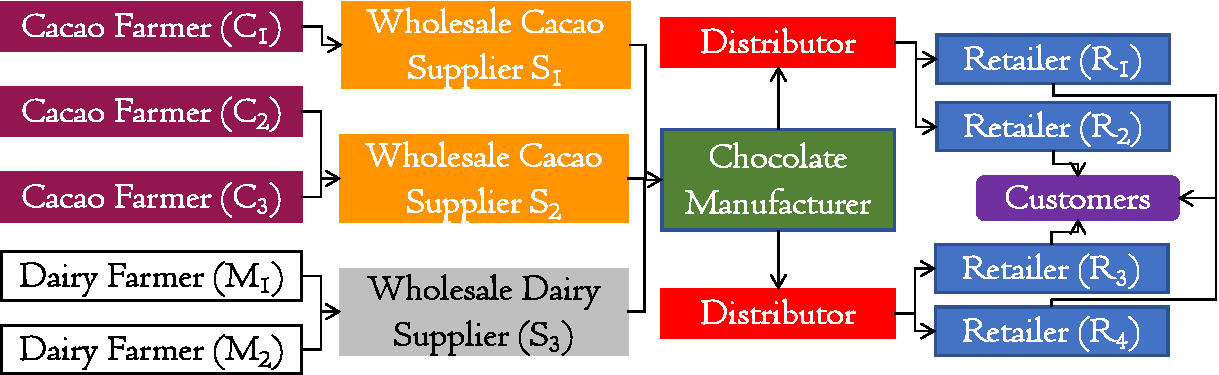
\includegraphics[scale=0.42]{fig/fsc.pdf}
  		\vspace{-.6cm}
		\caption{\small{Actors involved in a simplified food supply chain}.}
	    \label{fig:fsc}
 \end{center}
  \vspace{-.5cm}
\end{figure}
Figure~\ref{fig:fsc} shows actors involved in a simplified chocolate bars supply chain. For manufacturing a
chocolate bar, cacao and milk are required (assume a sugar free chocolate). Usually, manufacturers
buy raw materials from supplier rather than directly contacting various farmers. Once chocolate bars are produced,
via distributors, it would be sent to various retailers across the globe so that the chocolate bars can be sold
to customers. Note that distribution involes import/export authorities, customs and other entities. For simplicity,
we do not cover all involved actors.
\begin{figure}
    \begin{center}
	    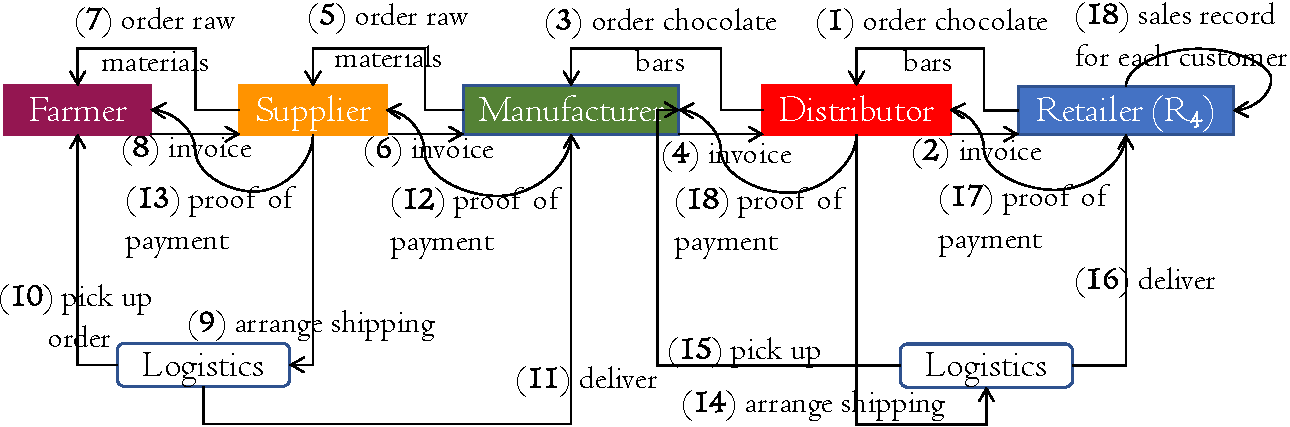
\includegraphics[scale=0.42]{fig/food-supply-chain-tx-flow.pdf}
  		\vspace{-.6cm}
		\caption{\small{A sample transaction flow in a chocolate supply chain}.}
	    \label{fig:tx-flow-fsc}
 \end{center}
  \vspace{-.5cm}
\end{figure}
Figure~\ref{fig:tx-flow-fsc} shows a sample business process in a chocolate supply chain. The process involves
order placement, invoice creation, shipping arrangement, delivery, and proof of payment. The whole process
can be implemented using a permissioned blockchain platform with the help of smart-contracts.
As blockchain is a replicated ledger, storing all information related to above process could leak
proprietary or business competitive information. For example, invoice details cannot be shared as it could leak
the business contract between the farmer and the supplier or the distributor and the retailer. As customer
contact details are very sensitive, it is not advisable to store it in the replicated ledger. However, storing
these details in a blockchain could help in resolving disputes and also it enables a tamper proof record
management for food traceability.
\par
For food traceability, actors don't need to store private/sensitive data in the replicate ledger instead can share information
on demand during an outbreak of food-borne illness. Further, storing the hash of private/sensitive data in the replicated
ledger would help in resolving disputes and tamper proof record management. Assume that a lot of customers are feeling ill due
to a food-borne disease, the food authority needs to find the list of food products each of these customers bought and then
trace it backward in the supply chain to start investigating the root cause. Similarly, it is easy for the actors to trace it
forward to recall potentially contaminated products.
\begin{figure}
    \begin{center}
	    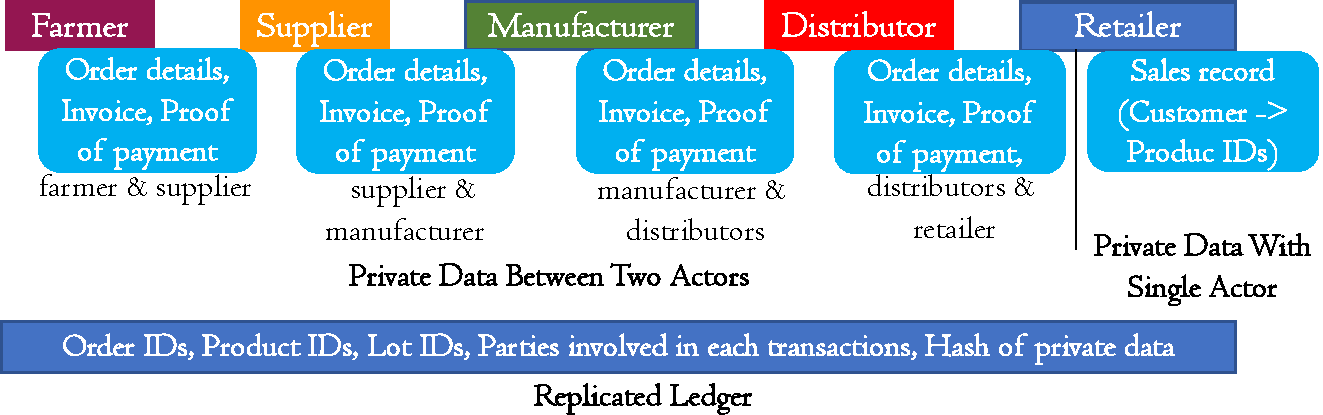
\includegraphics[scale=0.42]{fig/fsc-private-data.pdf}
  		\vspace{-.6cm}
		\caption{\small{Private data should not be shared with all participants as it could leak business contracts or other proprietary information}.}
	    \label{fig:fsc-pvt-data}
 \end{center}
  \vspace{-.5cm}
\end{figure}
\subsubsection{Existing Solutions and Drawbacks}
\par
\textbf{(1) Fabric Channel.}
\par
\textbf{(2) Quorum~\cite{} Private Transaction.}
\par
\textbf{(3) Encryption of Data.}
\par
\textbf{(4) Off-chain Storage With an On-chain Proof.}
\par
\textbf{(5) Zero Knowledge Proof.}
